\chapter{Background and Related Works}

%%%%%%%%%%%%%%%%%%%%%%%%%%%%%%%%%%%%%%%%%%%%%%%%%%%%%%%%%%%%%%%%%%%%%%%%%%%%%%%%%%%%%%%%%%%%%%%%%%%%

\section{ROS}

The \emph{Robot Operating System} (ROS) is an open-source framework for creating robot control systems, developed by \emph{Willow Garage} \cite{ros_paper}.

\subsection{Architecture}
ROS can be primarily thought of as a message-passing framework. A number of discrete processes, perhaps some even on a remote machine, communicate through a single broker service using an XMLRPC-based API. Each process performs a small part of a larger task, sharing data with other nodes through common data types.

Each resource has a unique name, and can be placed into a namespace. This gives each resource a unique \emph{graph resource name} which can be used to identify this resource elsewhere throughout the system. As the name suggests, the layout of a ROS system can be thought of as a graph or tree. Some examples of \emph{graph resource names} are shown below.

\begin{figure}[h]
    \centering

    \texttt{/} (the global namespace)

    \texttt{/hexapod} (the \emph{hexapod} namespace)

    \texttt{/hexapod/servo\_controller} (a \emph{servo\_controller} node)
\end{figure}

As touched on in the opening paragraph, ROS can function as a distributed system. Specifically, the processes can run on a machine different from that of the broker. The processes can then connect to the broker via a network. This can be used to offload complex computations onto another machine, should it be a requirement. To give an example, an embedded system running ROS on the robot can be collecting sensor data and issues hardware commands. This embedded system can then be communicating to a more powerful machine, acting as a base station. This base station can perform the more complex operations such as sensor data interpretation and path planning, relaying the commands back to the embedded system to be carried out.

\subsubsection{Nodes}
In ROS terminology, a processes is referred to as a \emph{node}. A node is simply a process that is connected to the ROS broker, performing some sort computation \cite{ros_paper}.

Nodes need not be tied to any particular programming language \cite{ros_paper}. Nodes are developed using a particular \emph{client library}, of which many are available. These are libraries developed for a particular language or ecosystem, providing an abstraction layer for interfacing with ROS. The two most used client libraries are \emph{roscpp} and \emph{rospy}, which target C++ and Python respectively \cite{ros_wiki_clientlibraries}. There are a number of experimental client libraries available for other systems, such as Java, Android, C\#, Arduino, among others \cite{ros_wiki_clientlibraries}.

\subsubsection{Communicating Through Topics \& Services}
Node communication is done through \emph{topics} in a one-to-many fashion \cite{ros_paper}. Broadcasting is done asynchronously, such that the broadcasting node can continue operating without regard as to which nodes receive the message. Any other node can then subscribe to that particular topic, receiving messages through a callback for processing. Each topic has a given resource name which is used to uniquely identify that topic.

A topic is defined with a given \emph{message} type. Messages are simple data structures consisting of a number of typed data fields. Each data field has a unique name, and can be of a number of built-in primitive types, as well as other arbitrarily nested data structures such as arrays and even other messages. A simple example of this would be the \texttt{Point} message from the \texttt{geometry\_msgs} package. This message consists of three \texttt{float64} fields named \texttt{x}, \texttt{y}, and \texttt{z} \cite{ros_api_point_msg}.

ROS also provides a \emph{request-response} style method of communication through \emph{services} \cite{ros_wiki_services}.

\subsubsection{Grouping Nodes in Packages}
A collection of nodes providing a particular set of functionalities (e.g., path planning for autonomous navigation), can be grouped and distributed as \emph{packages} \cite{ros_paper}. These packages can then be included into other projects acting as a subsystem as part of a larger system.

Users are encouraged to share and distribute any developments they make by hosting repositories of their code, preferably on \emph{GitHub} \cite{ros_wiki_getinvolved}. Contributors can then request that their repository be listed on a package index on the ROS website \cite{ros_wiki_getinvolved}. This aspect is a particular advantage of ROS, as there is a wide array of packages available for usage. Additionally, as ROS provides a number of common data types used in robotics, packages from different vendors can interact with one another with relative ease.

\subsection{Standard Packages \& Utilities}
\subsubsection{Launching Packages with roslaunch}
While nodes can launched manually, ROS provides a means for large sets of nodes programmatically via \emph{roslaunch} \cite{ros_paper, ros_wiki_roslaunch}. This tool allows developers to specify a set of nodes to be ran, along with a number of parameters, in XML configuration files ("launch files" in ROS terminology). \emph{roslaunch} provides many useful features.

A key feature is the ability to specify which namespace a particular set of nodes is in. This allows multiple nodes of the same type to be launched without conflict. Any topic used by a node can also be remapped to one more appropriate. This means that nodes can be built generically, assuming that their topics will be remapped to fulfil some specific purpose. An example of this is the \texttt{depthimage\_to\_laserscan} node, which converts a depth image into a format usable by nodes expecting laser scan data. This node expects the depth image to be transmitted on \texttt{/image}, assuming that this will be remapped to the actual depth image.

Launch files can also include other launch files. Generally, a package will provide a launch configuration that starts all the necessary nodes to provide dealing with this package. This can be used to create a "master" configuration that launches a number of necessary subsystems.

\subsubsection{Visualising Sensor Data with RViz}


%%%%%%%%%%%%%%%%%%%%%%%%%%%%%%%%%%%%%%%%%%%%%%%%%%%%%%%%%%%%%%%%%%%%%%%%%%%%%%%%%%%%%%%%%%%%%%%%%%%%

\section{Hardware}

The robotic hardware used in this project is relatively straightforward, consisting of a number of off-the-shelf components. The robot is a hexapod, in that it has six limbs. Each limb has three joints at which it can rotate, as shown in Figure~\ref{fig:hexapod_dof}, giving three degrees-of-freedom per limb. 

\begin{figure}[!h]
    \centering
    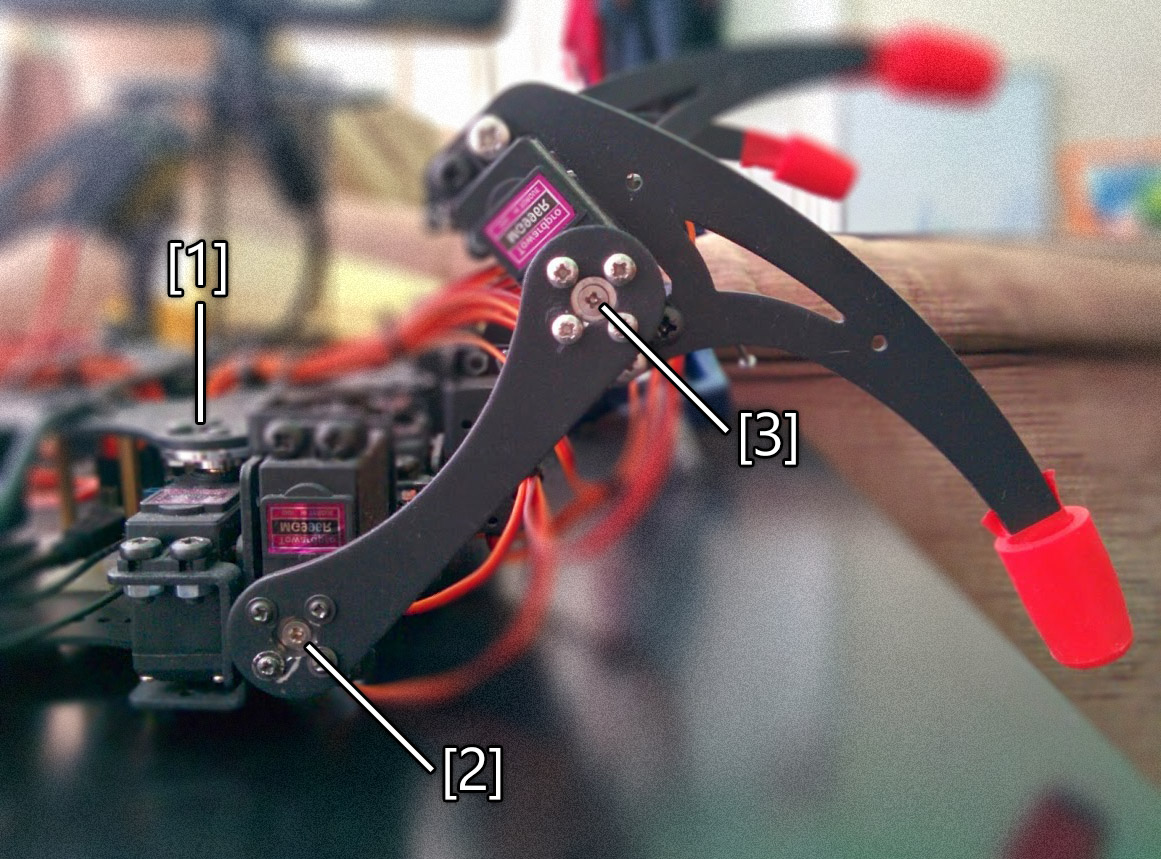
\includegraphics[width=10cm]{hexapod_joints}
    \caption{Joint 1 allows for horizontal rotation, whereas joint 2 and 3 allow for vertical rotation.}
    \label{fig:hexapod_dof}
\end{figure}

In its current state, the robot has no wireless capability and, thusly, operates in a tethered manner. A bundle of cables protruding from the rear end of the unit connects the on-board hardware to a nearby power source and computer.

\subsection{Servos \& Servo Controller}
Each joint piece is attached to the shaft of a servomechanism (servo) to facilitate rotation. Each servo is controlled by a \emph{pulse-width modulated} (PWM) signal supplied by the controller, such that the angle of the servo can be controlled. Servos operate using a feedback-loop system such that the current of a motor is controlled, rotating the shaft to the desired position. Rotational range and speed of servos vary depending on model, but in this case the servos allow for a total rotational range of 180\textdegree.

\begin{figure}[!h]
    \centering
    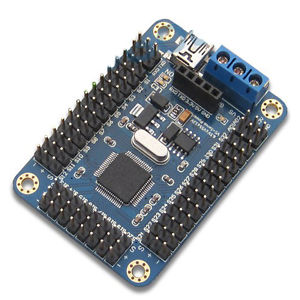
\includegraphics[width=6cm]{torobot_controller}
    \caption{The \emph{Torobot 32-Channel Servo Controller}, as used in the hexapod.}
    \label{fig:torobot_controller}
\end{figure}

The servos are controlled by an off-the-shelf servo controller board. This board, in particular, expects text-based control commands over serial, either via direct TTL or emulated over an on-board USB to TTL converter \cite{torobot_manual}. A number of commands are supported, allowing control of the position of both single and groups of servos. Additionally, a set of movements can be programmed and issues with a single command \cite{torobot_manual}. Power is also distrusted to the servos via this board.

\subsubsection{Protocol}

Commands are issues using an ASCII-based protocol via serial communication. While the servo controller supports a number of commands, only the command which rotates an individual servo is necessary. This allows for more flexibility in terms of when the rotation begins, as all servos mentioned in a group command will begin rotation at the same time.

\begin{figure}[!h]
    \centering
    \texttt{\#\(n\)\#P\(a\)T\(t\)\emph{\textbackslash r\textbackslash n}}
\end{figure}

A rotation command is issued by sending a string in the format shown above, specifying the particular servo number ($n$), the target angle ($a$), and the time over which the rotation should occur ($t$) in milliseconds. It should be noted that the parameter for the target angle is actually the pulse width duration that is sent to the servo, rather than the actual angle. Duration ranges can very per manufacturer, however there is a common standard such that 1.5\textmu s corresponds to 0\textdegree{} and 2.5\textmu s correspond to 180\textdegree. These are the minimum and maximum possible values for this controller.

\subsection{RGB-D Sensor}
The primary sensor in the system is an \emph{ASUS Xtion Pro Live} RGB-D sensor, which is very similar to the \emph{Microsoft Kinect}. The key functionality of this sensor is that it provides a depth video feed, giving a range of values indicating the distances to the objects in front of it.

Whole bunch of example pictures of how it works, what it does, etc.

The advantages this particular sensor provides over the \emph{Kinect} is mostly physical, specifically weight and footprint. The \emph{Kinect} has a motorized base which allows the device to be tilted upwards and downwards through software, in comparison to the \emph{Xtion} which has a simple hinge that can be rotated by hand. This feature is unnecessary in this use case and adds a significant amount of weight. Additionally, the \emph{Kinect} is intended to be a consumer device and, thus, has a much striking product design. However, this striking design comes at a cost of making the device much larger in general, which is somewhat troubling when it must be placed on an already space-starved robot base.

%%%%%%%%%%%%%%%%%%%%%%%%%%%%%%%%%%%%%%%%%%%%%%%%%%%%%%%%%%%%%%%%%%%%%%%%%%%%%%%%%%%%%%%%%%%%%%%%%%%%

\section{Existing Examples}